\documentclass{ctexart}
\usepackage{graphicx , geometry , float , subfigure , hyperref}
\geometry{a4paper , scale=0.85}


\title{Task 3 Report}
\author{2400012949 周诗城}
\date{}
\begin{document}
\maketitle
\section{Introduction}
In this task, I implemented a pytorch-like neural network framework Mytorch.
Almost all the components of the framework are implemented in C++ and cuda, including the tensor,
operator, autograd, optimizers. To be note, the Conv2d and GroupConv2d are implemented not only in im2col approach, 
but also in implicit gemm approach for memory efficiency. What's more, I implement the ResNet and ResNeXt in Mytorch.
They are both tested on CIFAR-10 and TinyImageNet datasets. I also implement saving and loading for models so that I can save 
the results for verification. You can find the code in github repository \url{https://github.com/ANinjaRabbit/Mytorch}.
\section{Structure}
First, I implement \textbf{TensorRaw} and \textbf{Tensor} templates to represent tensor-like data structure, where Tensor is just a 
shared-pointer version of TensorRaw.

Then, in namespace \textbf{nn}, I implement \textbf{modules} and \textbf{functions}, where modules typically have states and parameters, while functions doesn't. Every node 
in the computation graph we use in back propagation is connected with functions. However, for the sake of efficiency, I implemement back propagation for 
some modules like Linear and Conv. In this case, I use a wrapper called \textbf{ModuleFunctionWrapper} to wrap the module into a function (this function has 
side effects to update the internal parameters)

I also implement \textbf{ResNet} and \textbf{ResNeXt} in namespace \textbf{nn}.

In namespace \textbf{nn::optim}, I implement \textbf{optimizers} and \textbf{learning rate schedulers} to update the parameters of the model. We only implement two optimizers, 
\textbf{SGD with momentum} and \textbf{AdamW}, and two learning rate schedulers, \textbf{StepLR} and \textbf{CosineAnnealingLR}.

\section{Implementations}
All the implementations of modules are using pure cuda code. The Conv2d and GroupConv2d are implemented not only in im2col approach, 
but also in implicit gemm approach for memory efficiency. Finally, to achieve a balance between memory efficiency and computation efficiency and speed,
I use a mixed approach to implement Conv2d and GroupConv2d. For forward propagation and input gradient calculation, I use the implicit gemm approach, 
while for kernel gradient calculation, I use the im2col approach. The implementation of implicit gemm takes a lot of effort to optimize,
including using shared memory to reduce global memory access, using tile layout to avoid bank conflict, prefetching to avoid data dependency, epilogue to handle the bias. These codes can be find in 
nn.cu.

Note: the implementation of GroupConv2d and ResNeXt is experimental and not optimized. Using ResNeXt may be slower than ResNet. As a result, though we test both on CIFAR-10 and TinyImageNet, 
the hyperparameters of ResNeXt may be set improperly for speed, thus result in bad performance for ResNeXt.

\section{Experiments}
The approach we use for data augmentation is TrivialAugmentaion.
Both are using AdamW optimizer with CosineAnnealingLR scheduler.
The machine I use for training is a gaming desktop with RTX 4070 GPU, with 8GB VRAM.
\subsection{Cifar10}
I train these models using train\_cifar10.py.
The results are shown in following table. All the models are saved in models folder and can be verified by test\_cifar10.py

\begin{table}[H]
    \centering
    \begin{tabular}{|c|c|c|c|c|}
        \hline
        Model & Accuracy & Training Epochs & Training Time\\
        \hline
        ResNet18 & 92.31\% & 150 epochs & 5.5 hr \\
        \hline
        ResNeXt18 & 85.11\% & 150 epochs & 4.4hr \\
        \hline
    \end{tabular}
    \caption{Results on CIFAR-10}
    \label{tab:results_cifar10}
\end{table}

The speed of our framework is about one fourth of pytorch on ResNet18.

The accuracy and loss curve are shown in following figure.
\begin{figure}[H]
    \centering
    \subfigure[Accuracy curve of ResNet18 on CIFAR-10]{
        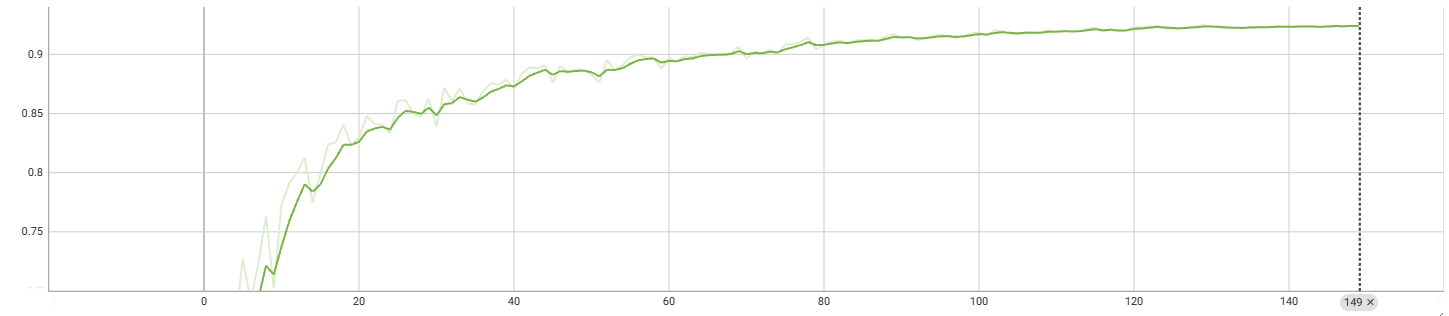
\includegraphics[width=0.45\textwidth]{cifarresnet18acc.png}
    }
    \subfigure[Loss curve of ResNet18 on CIFAR-10]{
        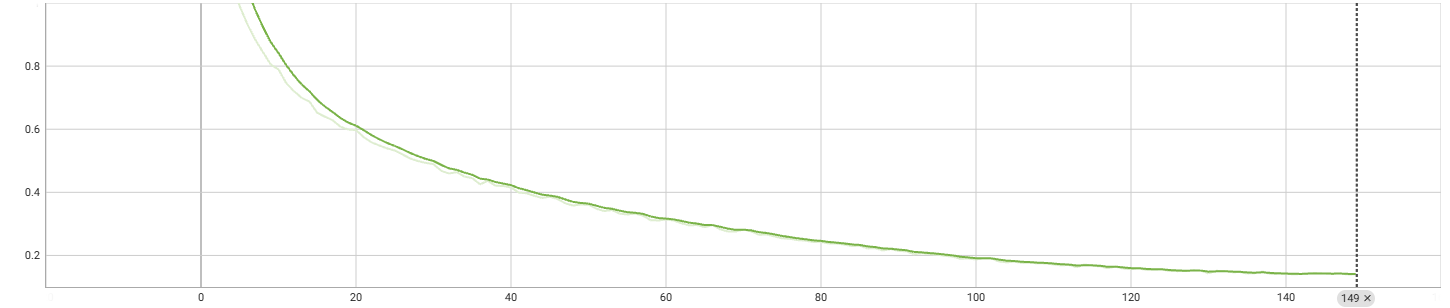
\includegraphics[width=0.45\textwidth]{cifarresnet18loss.png}
    }
    \subfigure[Accuracy curve of ResNeXt18 on CIFAR-10]{
        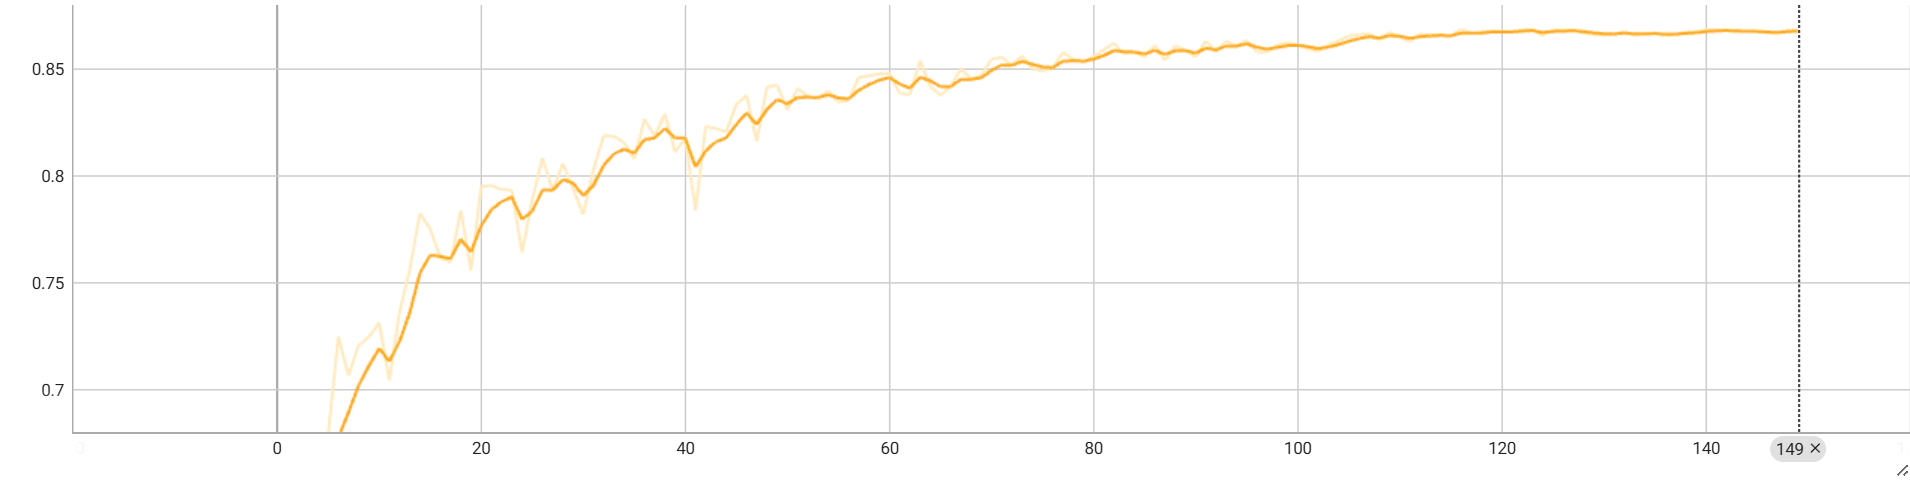
\includegraphics[width=0.45\textwidth]{cifarresnext18acc.png}
    }
    \subfigure[Loss curve of ResNeXt18 on CIFAR-10]{
        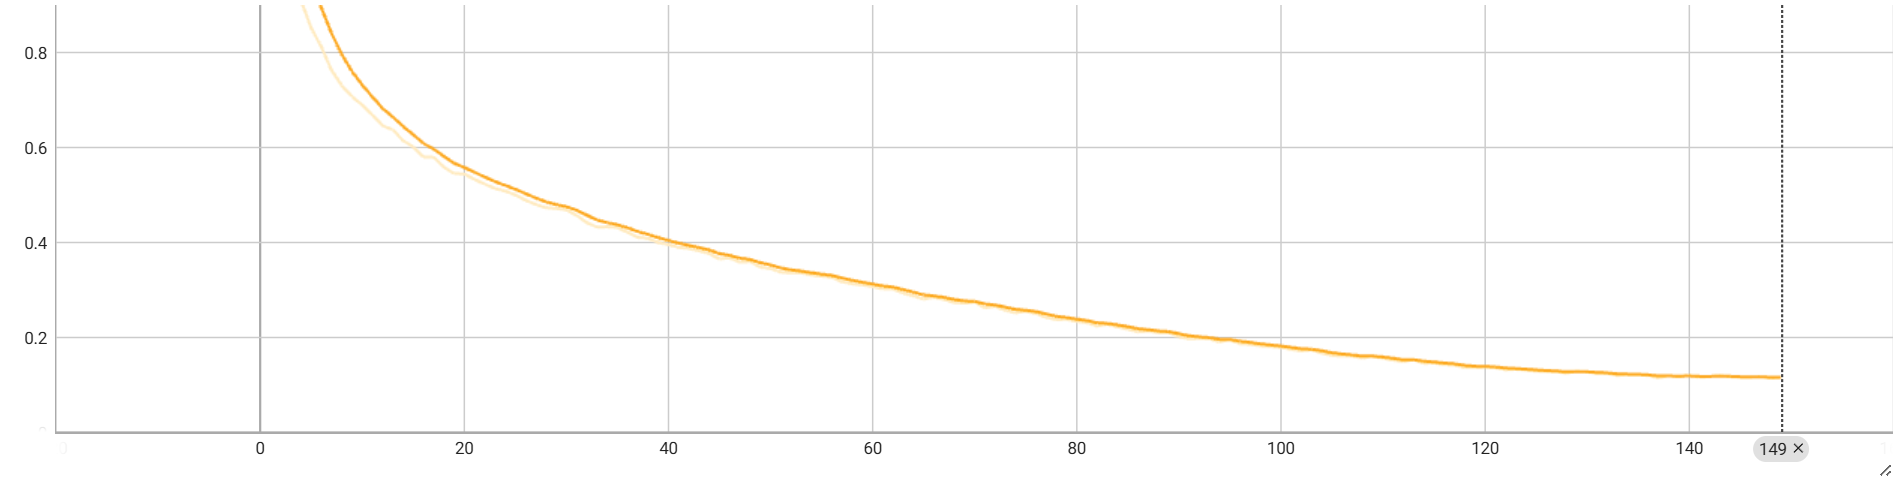
\includegraphics[width=0.45\textwidth]{cifarresnext18loss.png}
    }

\end{figure}

\subsection{TinyImageNet}
I choose Tiny ImageNet dataset for the bonus task. This dataset contains 200 classes of 64x64 images.
I train these models using train\_imagenet.py.
Resnet18 can achieve 57.94\% accuracy on TinyImageNet dataset, while ResNeXt18 can achieve 51.69\% accuracy.
All the models are saved in models folder and can be verified by test\_imagenet.py.

The results are shown in table below.
\begin{table}[H]
    \centering
    \begin{tabular}{|c|c|c|c|c|}
        \hline
        Model & Accuracy & Training Epochs & Training Time\\
        \hline
        ResNet18 & 57.94\% & 50 epochs & 10.63 hr \\
        \hline
        ResNeXt18 & 51.69\% & 50 epochs & 7.878 hr \\
        \hline
    \end{tabular}
    \caption{Results on TinyImageNet}
    \label{tab:results_tinyimagenet}
\end{table}

The accuracy and loss curve are shown in following figure.
\begin{figure}[H]
    \centering
    \subfigure[Accuracy curve of ResNet18 on TinyImageNet]{
        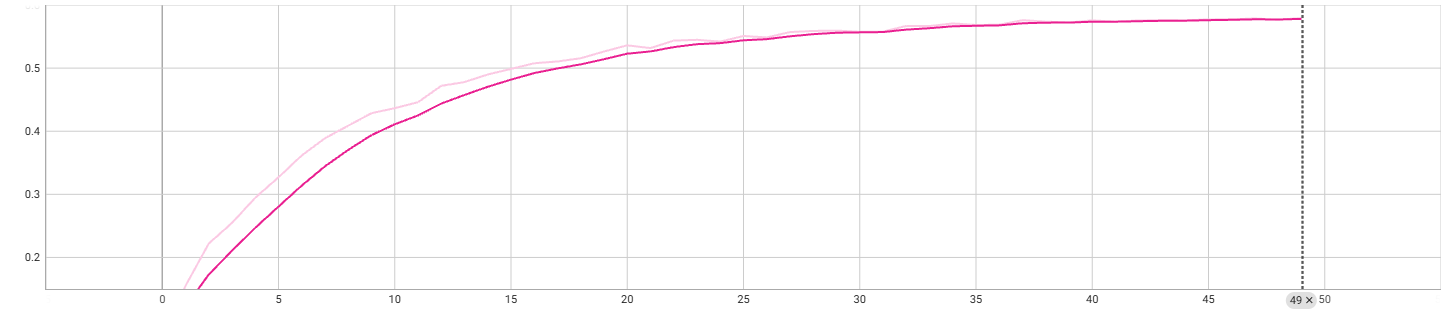
\includegraphics[width=0.45\textwidth]{tinyresnet18acc.png}
    }
    \subfigure[Loss curve of ResNet18 on TinyImageNet]{
        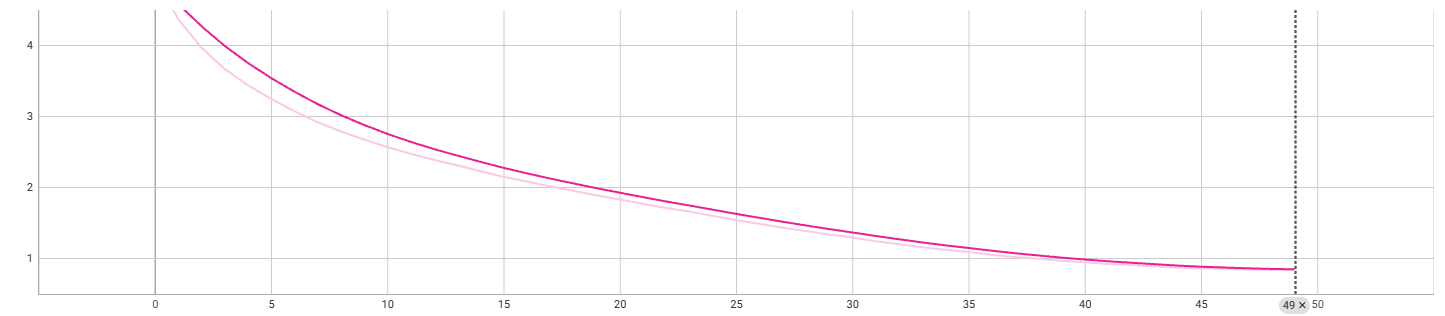
\includegraphics[width=0.45\textwidth]{tinyresnet18loss.png}
    }
    \subfigure[Accuracy curve of ResNeXt18 on TinyImageNet]{
        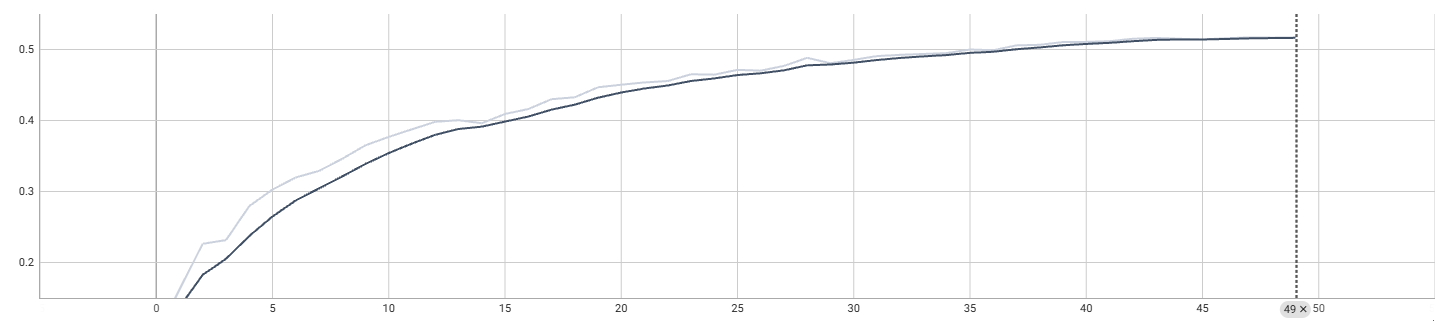
\includegraphics[width=0.45\textwidth]{tinyresnext18acc.png}
    }
    \subfigure[Loss curve of ResNeXt18 on TinyImageNet]{
        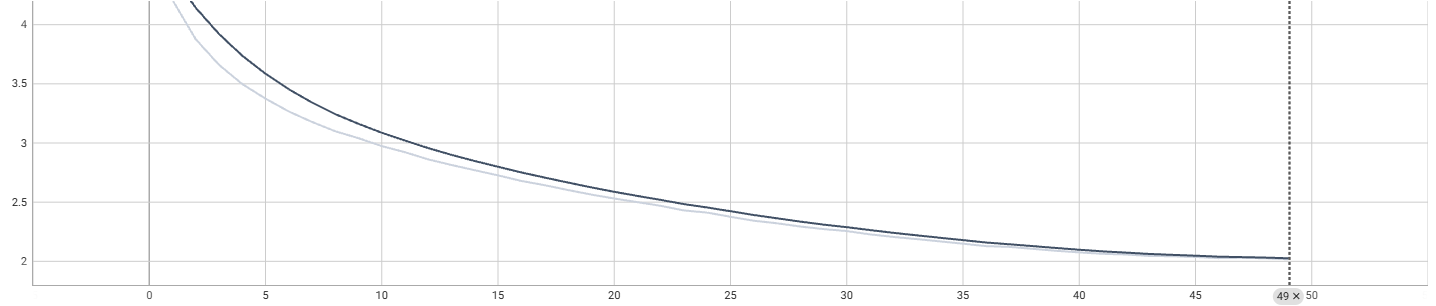
\includegraphics[width=0.45\textwidth]{tinyresnext18loss.png}
    }
\end{figure}

Note that although the whole training process takes 10.63 hours for ResNet18, 
The accuracy can achieve 50\% after 17 epochs and 3.64 hours.

The benchmark of several models on TinyImageNet is shown in following table.

\begin{table}[H]
    \centering
    \begin{tabular}{|c|c|}
        \hline
        Model & Accuracy \\
        \hline
        VGG16 & 57.45\%\\
        \hline
        ResNet18 & 54.039\%\\
        \hline
        ResNet34 & 54.601\%\\
        \hline
    \end{tabular}
    \caption{Benchmark of several models on TinyImageNet}
    \label{tab:benchmark_tinyimagenet}
\end{table}

We can see that our models achieve and compare well with the benchmark. This may be due to the TrivialAugmentaion
which is a simple and effective data augmentation method.








\end{document}